\documentclass{jsarticle}

\usepackage[dvipdfmx]{graphicx}
\usepackage{tabularx}
\usepackage{booktabs}
\usepackage[dvipdfmx]{xcolor}
\usepackage{listings} 
\usepackage{url}

\title{BBS掲示板の仕様書}
\author{24G1055 桑原拓也}
\date{}
\begin{document}
\maketitle
\section*{利用者向け}
掲示板を利用するには,サーバーが開いているとき,webブラウザで
\url{http://localhost:8080/public/bbs.html}にアクセスする.
アクセスすると図\ref{ex1}のような画面のサイトにアクセスされる.
掲示板では名前とメッセージの投稿,投稿の確認,投稿の削除・更新,投稿の検索
をすることができる.
\subsection*{機能の説明}
\noindent
・投稿機能は,名前の右の欄に掲示板で使用する名前を入力し,メッセージの右の欄に
投稿したい内容を入力し,送信ボタンを押すことで,サーバーに内容が送られる.\\
・投稿確認では,投稿チェックボタンを押すことで投稿された名前と内容,編集,削除が上に表示される.
複数投稿があった場合には新しく投稿された内容が前の投稿の下に表示されるようになっている.
例として,図\ref{ex2}はテストという名前でテストとメッセージを送信したものである.\\
・編集機能では,投稿された内容が表示された横に空欄のテキストボックスがあり,テキストボックスに
変更したい内容を入力し編集ボタンを押すことで,その投稿の内容をテキストボックスに書き込んだ内容に変更し投稿される.\\
・削除機能では,投稿された内容が表示された横に削除ボタンがあり,削除ボタンを押すことでその投稿を
消すことができる.投稿を削除した場合復元をすることはできない.\\
・検索機能では,キーワードを入力の右の欄に検索したい投稿内容の1部を入力し,
検索ボタンを押すことで,入力したキーワードの内容が含まれる投稿のみを表示する.
また,検索リセットボタンを押すと,もう一度すべての投稿を表示する.

\begin{figure}[h]
    \centering
    \begin{minipage}[b]{0.45\textwidth}
      \centering
      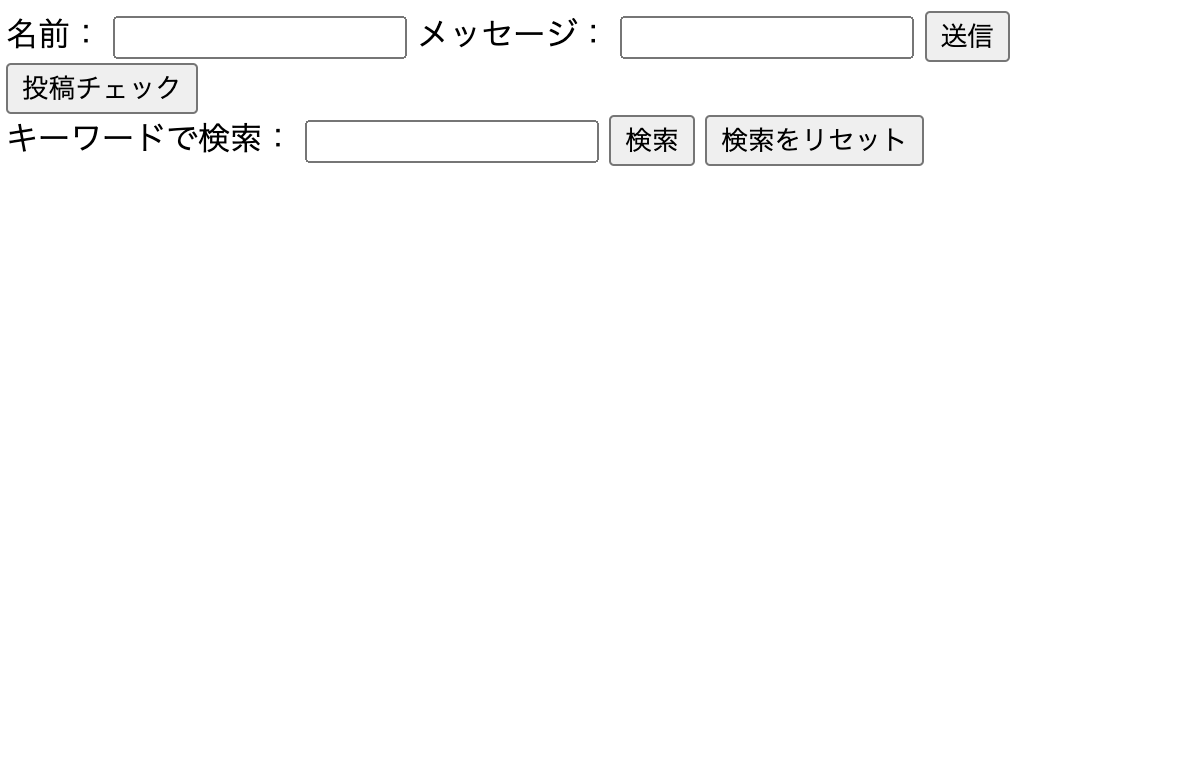
\includegraphics[height=45mm]{fig/ex1.png}
      \caption{掲示板のサイトの画面}
      \label{ex1}
    \end{minipage}
    \begin{minipage}[b]{0.45\textwidth}
      \centering
      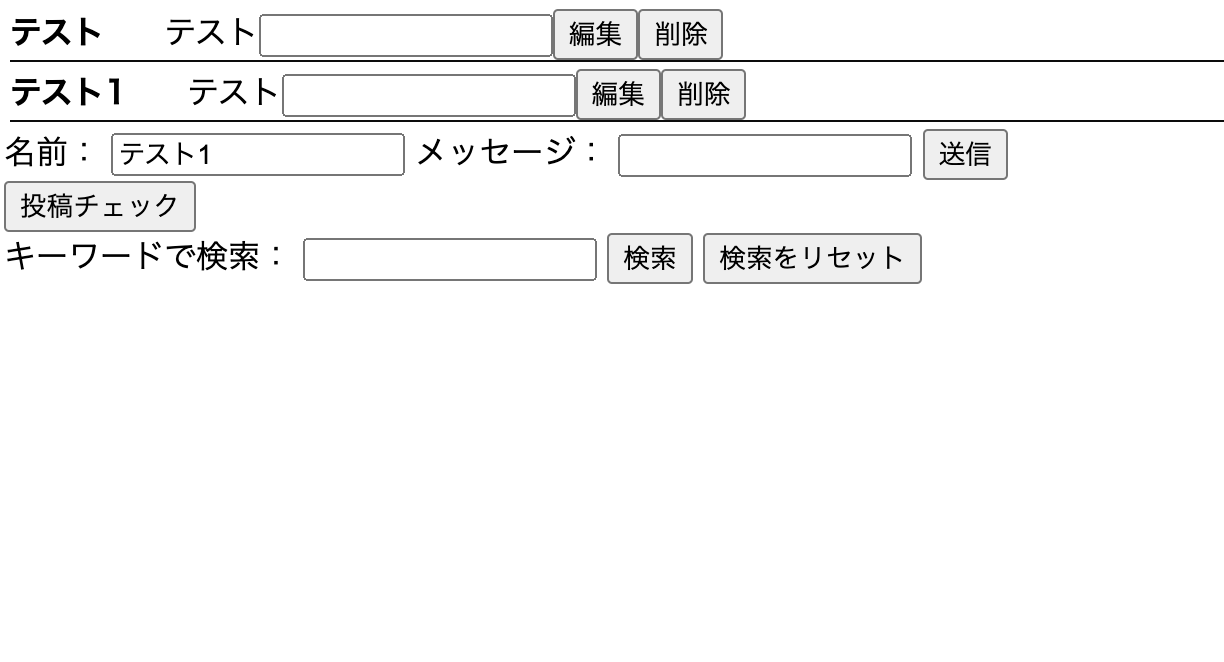
\includegraphics[height=45mm]{fig/ex2.png}
      \caption{投稿を表示した例}
      \label{ex2}
    \end{minipage}
\end{figure}

\clearpage
\section*{管理者向け}
掲示板を使用するに当たってプログラムの書かれたサーバーを起動する必要がある.
掲示板のサーバーを起動するのに必要なファイルは,表\ref{file}に示す4つのファイルである.
サーバーの起動方法は,まずターミナルを起動しプログラムの入った適切なファイルに移動する.
次に,ターミナルでnode app7.jsを入力し掲示板のサーバーを起動する.
ソースコードのファイルは\url{https://github.com/KuwabaraTakuya/webpro_06}のgithub内に置いてある.

\begin{table}[ht]\caption{掲示板のファイル一覧}
    \centering
    \begin{tabular}{|c|c|}
       \hline
       ファイル名 &  説明  \\ 
        \hline
        app7.js  & サーバーのプログラム  \\ \hline
        public/bbs.js  & クライアントのプログラム  \\ \hline
        public/bbs.html & 掲示板の表示画面\\ \hline
        public/bbs.css &  HTMLのスタイルシート \\ \hline
    \end{tabular}
    \label{file}
\end{table}
    
\clearpage
\section*{開発者向け}
\subsection*{プログラムの概要}
この掲示板は,テキストを書き込みボタンをクリックすることによってサーバーとクライアント
の双方向でデータを送受信し,テキストを保存したり,表示させたり,編集・削除したりするプログラムである.
図\ref{システム}は,掲示板システムの全体の流れを表したものである.
webブラウザでwebページを取得したあとは,BBSクライアントとBBSサーバ
が双方向でデータを送受信することでシステムができている.
掲示板システムのソースコードのファイルは\url{https://github.com/KuwabaraTakuya/webpro_06}のgithub内に置いてある.
\begin{figure}[h]
    \centering
    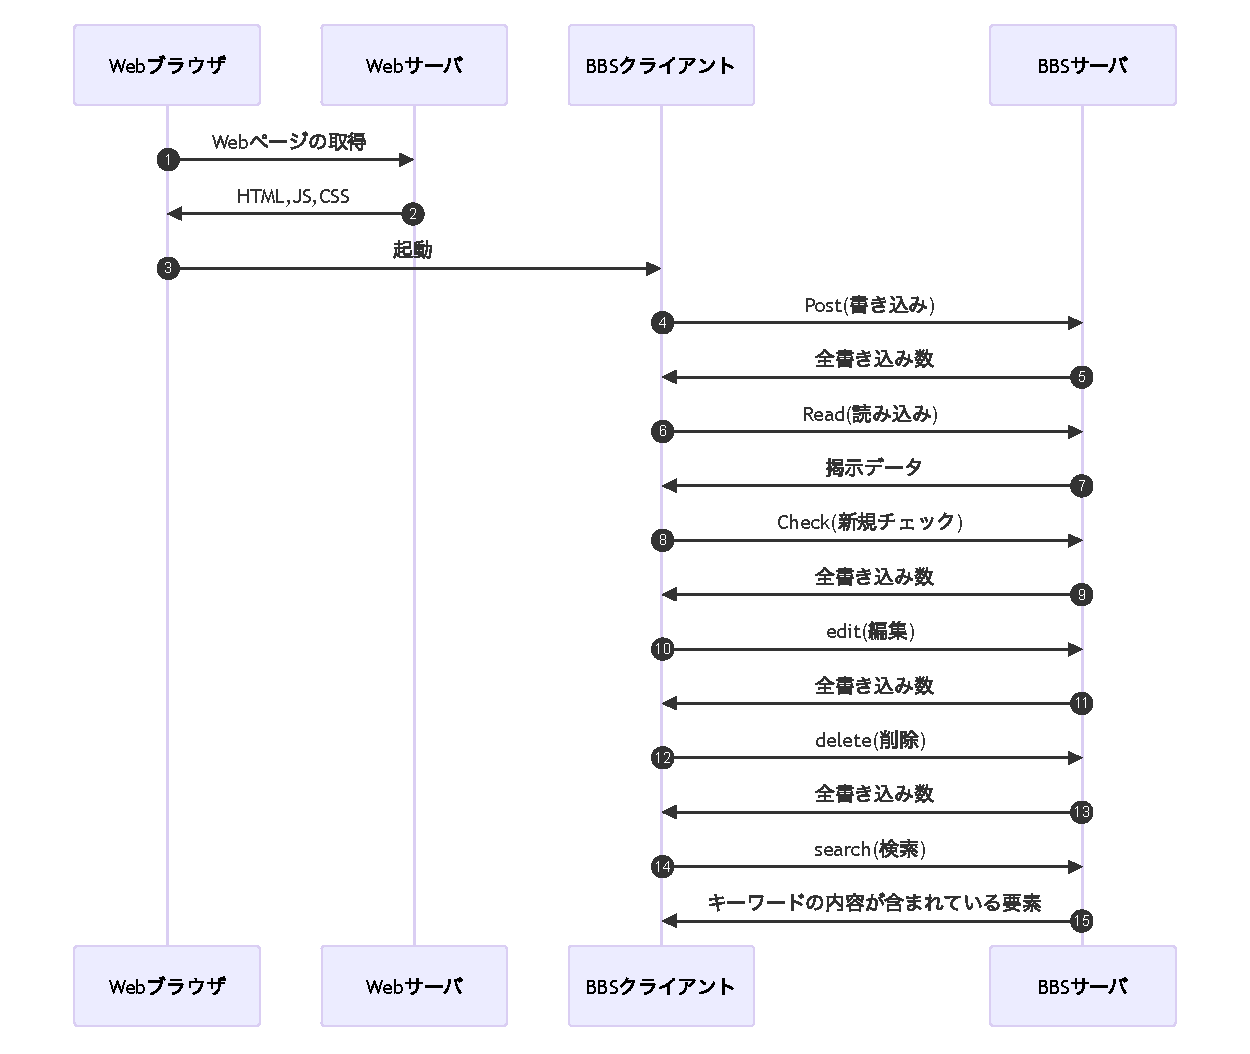
\includegraphics[width=120mm]{fig/system.pdf}
    \caption{掲示板システム全体の流れ}
    \label{システム}
\end{figure}
\subsection*{プログラムの詳細}
\subsubsection*{送信ボタンを押したときの流れ}
まずクライアント側でメッセージの書き込みされた内容を
受け取り,POSTメソッドを使用しbodyに受け取った内容を格納しサーバーへと送信する.サーバーでは
bodyの内容を受け取り,bbsの配列の中に格納する.このとき,bbsの長さをidとしてbbsの中に格納する.
そしてサーバー側からjson形式でクライアント側にbbsの長さを返す.
クライアント側はbbsの長さを受け取ったら,メッセージを書き込むテキストボックスを空にする.

\begin{table}[ht]\caption{送信の際に使用した変数}
    \centering
    \begin{tabular}{|c|c|}
       \hline
       変数名 &  説明  \\ 
        \hline
        bbs  &  名前,投稿内容,idの保存\\ \hline
        name &  入力された名前の記録  \\ \hline
        message  & 入力された投稿内容の記録  \\ \hline
        params& HTTPリクエストの詳細 \\ \hline
        id &  bbsの配列の長さを記録 \\ \hline
    \end{tabular}
    \label{post}
\end{table}


\subsubsection*{投稿チェックボタンを押したときの流れ}
まずクライアント側でPOSTメソッドを使用しサーバーへと送信する.
サーバーでは,json形式でbbsの長さをクライアントへ返す.
bbsの長さを受け取り,bbsの長さとnumber違った場合,POSTメソッドを使用しbodyにnumberを格納し
サーバーへと送信する.
サーバーでは,numberを受け取り0であればjson形式でbbsを返し,そうでなければjson形式でbbsの配列のnumber番目から最後までを
クライアントへ返す.
クライアント側でbbsを受け取り,bbsに格納されていた名前とメッセージを表示させる.
このとき編集するためのテキストボックスとボタン,削除するためのボタンを表示させ,onclickによって
ボタンを押したときぞれぞれの機能を実行する関数を呼び出すように設定した.
onclickは,HTML要素に対してクリックイベントを監視し,そのイベントが発生したときに,
値として関数を代入することで動作を指定できるものである.onclickを使うことで,1つ1つのボタンに別のid
を割り振らずに対象の投稿に動作させることができるため採用した.

\begin{table}[ht]\caption{投稿チェックの際に使用した変数}
    \centering
    \begin{tabular}{|c|c|}
       \hline
       変数名 &  説明  \\ 
        \hline
        bbs  &  名前,投稿内容,idの保存\\ \hline
        number   & これまで読み込んだ投稿の数  \\ \hline
        params& HTTPリクエストの詳細 \\ \hline
        cover &  各投稿をdiv.coverの中にまとめる \\ \hline
        name\_area& 投稿者の名前表示のためのspan要素 \\ \hline
        mes\_area& 投稿内容表示のためのspan要素\\ \hline
        edit\_area& 編集内容を書き込むためのテキストボックス\\ \hline
        edit\_button& 編集するためのボタン要素\\ \hline
        delete\_button& 削除するためのボタン要素\\ \hline
    \end{tabular}
    \label{check}
\end{table}


\subsubsection*{編集ボタンを押したときの流れ}
編集ボタンを押したときonclickによってeditPost関数を呼び出す.
このとき,編集のテキストボックスの内容とbbsに格納されていたidを引数とする.
まずクライアント側でPOSTメソッドを使用しbodyに編集のテキストボックスの内容を格納しサーバーへと送信する.
サーバーでは,編集のテキストボックスの内容とidを受け取り,bbsの配列の中のidが同じ要素を取り出し,その要素のメッセージを
編集のテキストボックスの内容に変更し,json形式でbbsの長さをクライアントへ返す.
クライアント側はbbsの長さを受け取ったら,HTMLを空にしてnumberを0にしてから
投稿チェックをすることで,すべての投稿を再読込して編集した内容を
表示させる.
bbsの配列の中のidが同じ要素を取り出すためfind()を使用した.
find()とは関数を満たす配列内の最初の要素を返すメソッドである.

\begin{table}[ht]\caption{編集の際に使用した変数}
    \centering
    \begin{tabular}{|c|c|}
       \hline
       変数名 &  説明  \\ 
        \hline
        bbs  &  名前,投稿内容,idの保存\\ \hline
        id &  メッセージのidの記録  \\ \hline
        newMessage  & 編集内容の記録  \\ \hline
        params& HTTPリクエストの詳細 \\ \hline
        post &  bbs内に同じidを持つ要素 \\ \hline
        number   & これまで読み込んだ投稿の数  \\ \hline
    \end{tabular}
    \label{edit}
\end{table}


\subsubsection*{削除ボタンを押したときの流れ}
編集ボタンを押したときonclickによってdeletePost関数を呼び出す.
このとき,bbsに格納されていたidを引数とする.
まずクライアント側でPOSTメソッドを使用しサーバーへと送信する.
サーバーでは,編集のテキストボックスの内容とidを受け取り,bbsの配列の中のidが同じ要素を取り出し,その要素を配列から
取り除き,json形式でbbsの長さをクライアントへ返す.
クライアント側はbbsの長さを受け取ったら,HTMLを空にしてnumberを0にしてから
投稿チェックをすることで,すべての投稿を再読込して編集した内容を
表示させる.

\begin{table}[ht]\caption{削除の際に使用した変数}
    \centering
    \begin{tabular}{|c|c|}
       \hline
       変数名 &  説明  \\ 
        \hline
        bbs  &  名前,投稿内容,idの保存\\ \hline
        id &  メッセージのidの記録  \\ \hline
        params& HTTPリクエストの詳細 \\ \hline
        post &  bbs内に同じidを持つ要素 \\ \hline
        number   & これまで読み込んだ投稿の数  \\ \hline
    \end{tabular}
    \label{delete}
\end{table}


\subsubsection*{検索ボタンを押したときの流れ}
まずクライアント側で検索するためのキーワードの内容を受け取り,POSTメソッドを使用し
bodyに受け取った内容を格納しサーバーへと送信する.
サーバーでは,bbsの配列の中からキーワードの内容が含まれている内容を取り出し,その要素をjson形式でクライアントへ返す.
クライアント側はキーワードの内容が含まれている要素を受け取り,HTMLを空にしてから要素に含まれる
名前とメッセージを表示する.
また,検索リセットボタンを押すとHTMLを空にしてnumberを0にしてから投稿チェック
をすることで,すべての投稿を再読込して編集した内容を表示させる.
bbsの配列の中からキーワードの内容が含まれている内容を取り出す際に,filter()とincludes()を使用した.
includes()は,配列において特定の値が含まれているかどうかを判定するためのメソッドであり,今回では,
キーワードの内容がbbs内のメッセージに含まれているかを判別するため採用した.
filter()は特定の条件の中で配列内の要素をフィルタリングし,新しい配列として返す
メソッドである.今回では,配列の中にキーワードを含む要素をフィルタリングして,新しい配列として返すことで
キーワードを含む内容だけを表示させるため採用した.

\begin{table}[ht]\caption{検索の際に使用した変数}
    \centering
    \begin{tabular}{|c|c|}
       \hline
       変数名 &  説明  \\ 
        \hline
        bbs  &  名前,投稿内容,idの保存\\ \hline
        keyword &  検索キーワードの記録  \\ \hline
        params& HTTPリクエストの詳細 \\ \hline
        results &  bbs内に同じメッセージを含む要素 \\ \hline
        number   & これまで読み込んだ投稿の数  \\ \hline
    \end{tabular}
    \label{search}
\end{table}

\end{document}
